\chapter*{ANTON-BIVENS-DAVIS 9.7 EJERCICIO 29}

\textbf{29)} Encuentra los primeros 4 polinomios distintos de Taylor sobre $x = x_{0}$, y usa una utilidad gráfica para graficar la función dada y el polinomio de Taylor en la misma pantalla. \\
\begin{center}
   $f(x) = cos x$ en $  x_{0}= \pi$
\end{center}
Para facilitar la búsqueda de estos polinomios, primero hallemos las derivadas (que presentará una forma cíclica):
\begin{multicols}{3}
	\noindent
	\begin{align*}
		\text{Derivando: } &        \\
		f^{0}(x) =& cos(x) \\
        f^{1}(x) =& -sen(x) \\
        f^{2}(x) =& -cos(x) \\
        f^{3}(x) =& sen(x) \\
	\end{align*}
	\columnbreak
	\begin{align*}
		\text{Evaluando en: }& x_{0} = \pi     \\
		f^{0}(\pi) =& cos(\pi) \\
        f^{1}(\pi) =& -sen(\pi) \\
        f^{2}(\pi) =& -cos(\pi) \\
        f^{3}(\pi) =& sen(\pi) \\
	\end{align*}
	\columnbreak
	\begin{align*}
		\text{Valor: }&      \\
        cos(\pi) =& -1\\
        -sen(\pi) =&  0\\
        -cos(\pi) =&  1\\
        sen(\pi) =&   0\\
	\end{align*}
\end{multicols}
Para generar los diferestes polinomios ocuparemos el desarrollo de Taylor:
\begin{align*}
   \sum_{k=0}^{n} \frac{f^{k}(x_{0})}{k!}(x-x_{0})^{k}
\end{align*}

Para $P_{0}(x)$ :
\begin{align*}
   \sum_{k=0}^{0} \frac{f^{k}(x_{0})}{k!}(x-x_{0})^{k} &= \frac{f^{0}(\pi)}{0!}(x-\pi)^{0} \\
   \frac{f^{0}(\pi)}{0!}(x-\pi)^{0}                    &= \frac{cos(\pi)}{1}(x-\pi)^{0} \\
   \frac{cos(\pi)}{1}(x-\pi)^{0}                       &= cos(\pi)(1) \\
   cos(\pi)(1)                                         &= -1 \\
\end{align*}
Así, esta es nuestra \textbf{primera} aproximación a la función. $P_{0}(x) = -1$ \\
Para $P_{1}(x)$ :
\begin{align*}
   \sum_{k=0}^{1} \frac{f^{k}(x_{0})}{k!}(x-x_{0})^{k} &= \frac{f^{0}(\pi)}{0!}(x-\pi)^{0} + \frac{f^{1}(\pi)}{1!}(x-\pi)^{1}\\
\end{align*}
Para el nuevo Término:
\begin{align*}
   \frac{f^{1}(\pi)}{1!}(x-\pi)^{1}                    &= \frac{-sen(\pi)}{1}(x-\pi) \\
   \frac{sen(\pi)}{1}(x-\pi)                           &= sen(\pi)(x-\pi) \\
   sen(\pi)(x-\pi)                                     &= 0 \\
\end{align*}
Así la sumatoria resulta:
\begin{align*}
   \sum_{k=0}^{1} \frac{f^{k}(x_{0})}{k!}(x-x_{0})^{k} &= -1 + 0\\
   \sum_{k=0}^{1} \frac{f^{k}(x_{0})}{k!}(x-x_{0})^{k} &= -1 \\
\end{align*}
En este caso podemos ver que dada la multiplación por 0 (debido a $sen(\pi)$) el polinomio resultante es igual al anterior (NO es distinto). \\
Podremos ver que se repetirá este comportamiento siempre que el término de la sumatoria involucre  $sen(\pi)$, con esto el término se "cancelará". \\

Para $P_{2}(x)$ :
\begin{align*}
   \sum_{k=0}^{2} \frac{f^{k}(x_{0})}{k!}(x-x_{0})^{k} &= \frac{f^{0}(\pi)}{0!}(x-\pi)^{0} + \frac{f^{1}(\pi)}{1!}(x-\pi)^{1} + \frac{f^{2}(\pi)}{2!}(x-\pi)^{2}\\
\end{align*}
Para el nuevo Término:
\begin{align*}
   \frac{f^{2}(\pi)}{2!}(x-\pi)^{2}                    &= \frac{-cos(\pi)}{2}(x-\pi)^{2} \\
   \frac{-cos(\pi)}{2}(x-\pi)^{2}                      &= \frac{1}{2}(x-\pi)^{2}\\
   \frac{1}{2}(x-\pi)^{2}                              &= \frac{(x-\pi)^{2}}{2}\\
\end{align*}
Así la sumatoria resulta:
\begin{align*}
   \sum_{k=0}^{2} \frac{f^{k}(x_{0})}{k!}(x-x_{0})^{k} &= -1 + \frac{(x-\pi)^{2}}{2}\\
\end{align*}
Así, esta es nuestra \textbf{segunda} aproximación a la función. $P_{2}(x) = -1 + \frac{(x-\pi)^{2}}{2}$ \\

Para $P_{3}(x)$ :
\begin{align*}
   \sum_{k=0}^{3} \frac{f^{k}(x_{0})}{k!}(x-x_{0})^{k} &= \frac{f^{0}(\pi)}{0!}(x-\pi)^{0} + \frac{f^{1}(\pi)}{1!}(x-\pi)^{1} + \frac{f^{2}(\pi)}{2!}(x-\pi)^{2} + \frac{f^{3}(\pi)}{3!}(x-\pi)^{3}\\
\end{align*}
Para el nuevo Término: \\
Como se mecionó mas arriba sabemos que el nuevo termino involucrará a $sen(\pi)$ (Dado que la derivación de $cos(x)$ es cíclica), por esto, este término también será 0. \\
\newline
Así la sumatoria resulta:
\begin{align*}
   \sum_{k=0}^{3} \frac{f^{k}(x_{0})}{k!}(x-x_{0})^{k} &= -1 + \frac{(x-\pi)^{2}}{2} + 0\\
   \sum_{k=0}^{3} \frac{f^{k}(x_{0})}{k!}(x-x_{0})^{k} &= -1 + \frac{(x-\pi)^{2}}{2} \\
\end{align*}
Por lo tanto este no es un Polinomio Distinto. \\

Para $P_{4}(x)$ :
\begin{align*}
   \sum_{k=0}^{4} \frac{f^{k}(x_{0})}{k!}(x-x_{0})^{k} &= \frac{f^{0}(\pi)}{0!}(x-\pi)^{0} + \frac{f^{1}(\pi)}{1!}(x-\pi)^{1} + \frac{f^{2}(\pi)}{2!}(x-\pi)^{2} + \frac{f^{3}(\pi)}{3!}(x-\pi)^{3}  + \frac{f^{4}(\pi)}{4!}(x-\pi)^{4}\\
\end{align*}
Para el nuevo Término:
\begin{align*}
   \frac{f^{4}(\pi)}{4!}(x-\pi)^{4}                    &= \frac{cos(\pi)}{24}(x-\pi)^{4} \\
   \frac{cos(\pi)}{24}(x-\pi)^{4}                      &= \frac{-1}{24}(x-\pi)^{4}\\
   \frac{-1}{24}(x-\pi)^{4}                              &= -\frac{(x-\pi)^{4}}{24}\\
\end{align*}
Así la sumatoria resulta:
\begin{align*}
   \sum_{k=0}^{4} \frac{f^{k}(x_{0})}{k!}(x-x_{0})^{k} &= -1 + \frac{(x-\pi)^{2}}{2} -\frac{(x-\pi)^{4}}{24}\\
\end{align*}
Así, esta es nuestra \textbf{tercera} aproximación a la función. $P_{4}(x) = -1 + \frac{(x-\pi)^{2}}{2} -\frac{(x-\pi)^{4}}{24}$ \\

Para $P_{5}(x)$ :
\begin{align*}
   \sum_{k=0}^{3} \frac{f^{k}(x_{0})}{k!}(x-x_{0})^{k} &= \frac{f^{0}(\pi)}{0!}(x-\pi)^{0} + \frac{f^{1}(\pi)}{1!}(x-\pi)^{1} + ....  + \frac{f^{5}(\pi)}{5!}(x-\pi)^{5}\\
\end{align*}
Para el nuevo Término: \\
Este termino también involucrará a $sen(\pi)$, por esto, este término también será 0. \\
\newline
Así la sumatoria resulta:
\begin{align*}
  \sum_{k=0}^{5} \frac{f^{k}(x_{0})}{k!}(x-x_{0})^{k} &= -1 + \frac{(x-\pi)^{2}}{2} -\frac{(x-\pi)^{4}}{24} + 0\\
  \sum_{k=0}^{5} \frac{f^{k}(x_{0})}{k!}(x-x_{0})^{k} &= -1 + \frac{(x-\pi)^{2}}{2} -\frac{(x-\pi)^{4}}{24}\\
\end{align*}
Por lo tanto este no es un Polinomio Distinto. \\

Para $P_{6}(x)$ :
\begin{align*}
   \sum_{k=0}^{6} \frac{f^{k}(x_{0})}{k!}(x-x_{0})^{k} &= \frac{f^{0}(\pi)}{0!}(x-\pi)^{0} + \frac{f^{1}(\pi)}{1!}(x-\pi)^{1} + ... + \frac{f^{6}(\pi)}{6!}(x-\pi)^{6}\\
\end{align*}
Para el nuevo Término:
\begin{align*}
   \frac{f^{6}(\pi)}{6!}(x-\pi)^{6}                    &= \frac{-cos(\pi)}{720}(x-\pi)^{6} \\
   \frac{-cos(\pi)}{720}(x-\pi)^{6}                      &= \frac{1}{720}(x-\pi)^{6}\\
   \frac{1}{720}(x-\pi)^{6}                              &= \frac{(x-\pi)^{6}}{720}\\
\end{align*}
Así la sumatoria resulta:
\begin{align*}
   \sum_{k=0}^{4} \frac{f^{k}(x_{0})}{k!}(x-x_{0})^{k} &= -1 + \frac{(x-\pi)^{2}}{2} -\frac{(x-\pi)^{4}}{24} + \frac{(x-\pi)^{6}}{720}\\
\end{align*}
Así, esta es nuestra \textbf{cuarta} aproximación a la función. $P_{6}(x) = -1 + \frac{(x-\pi)^{2}}{2} -\frac{(x-\pi)^{4}}{24} + \frac{(x-\pi)^{6}}{720}$ \\
\newline
Podemos notar comportamientos similares en las aproximaciones con lo cual incluso Podríamos generar una fórmula para generar estos Polinomio. \\
\newline
\textbf{A continuación están las gráficas, tanto de la función original como de los Polinomios Generados:} \\

\begin{figure*}
    \centering
    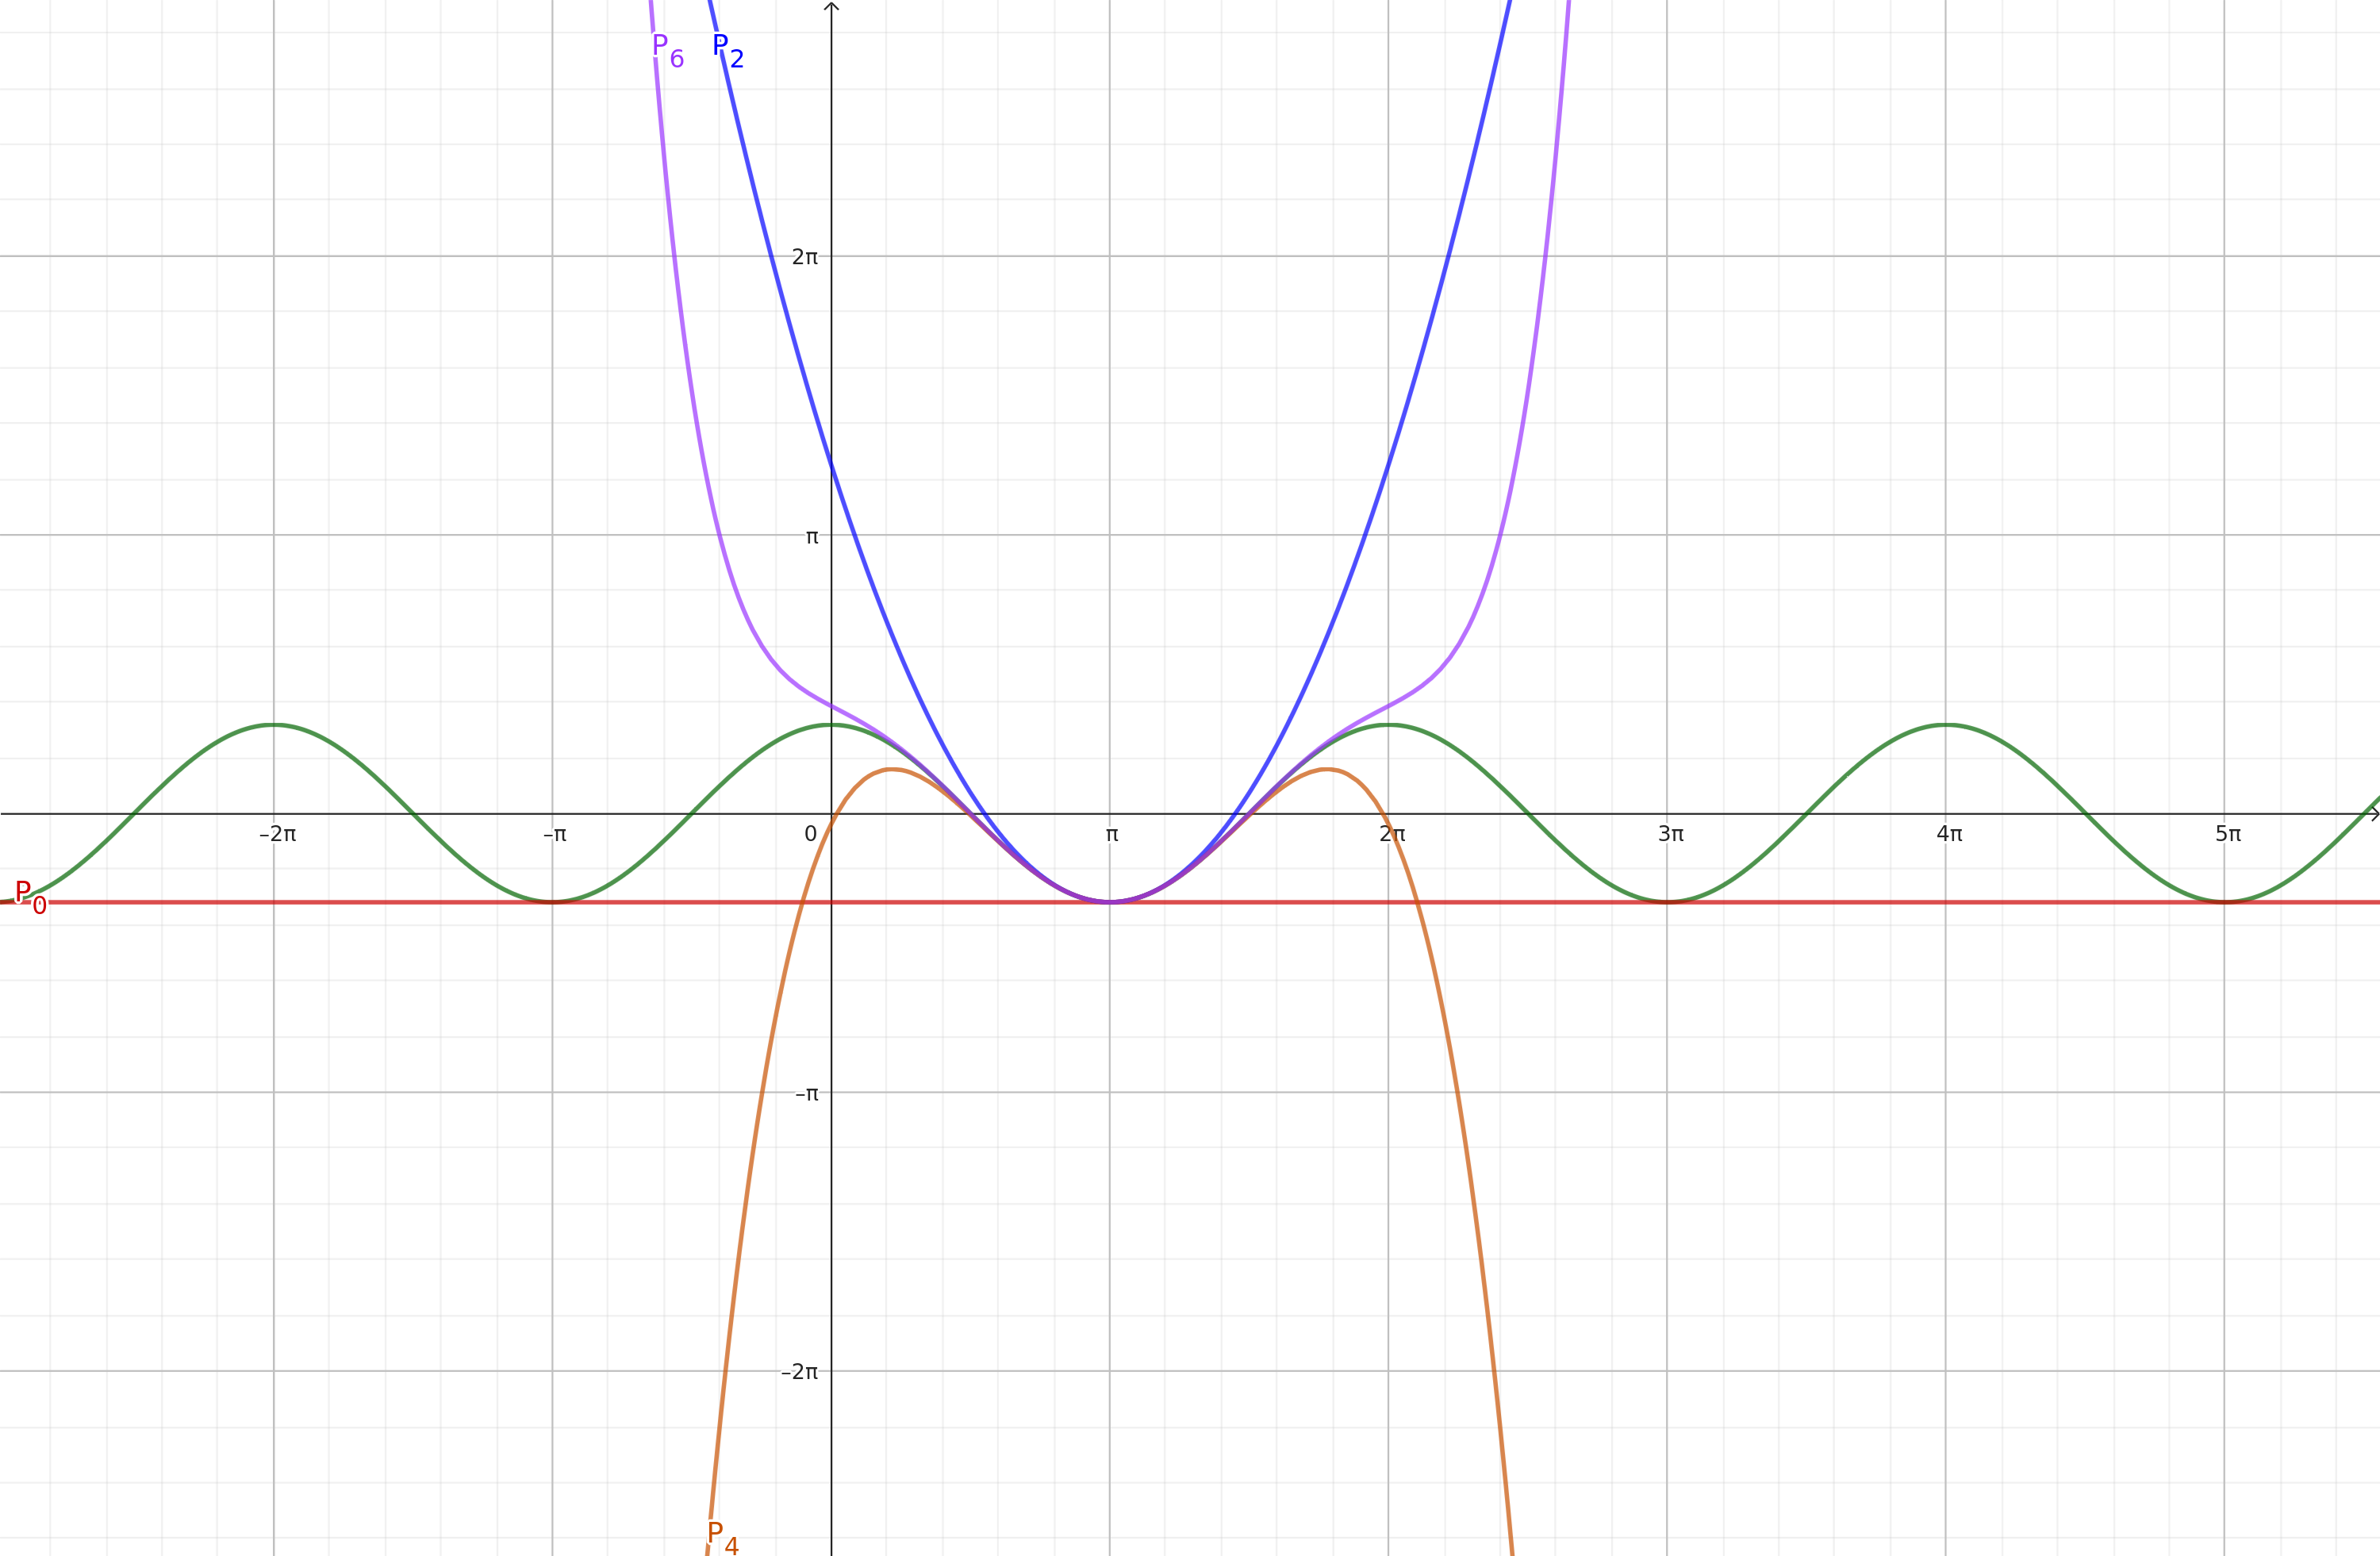
\includegraphics[height = 0.25\textheight]{recursos/polinomios/29.png}\par
    \caption*{Gráfica de la función y los Polinomios}
    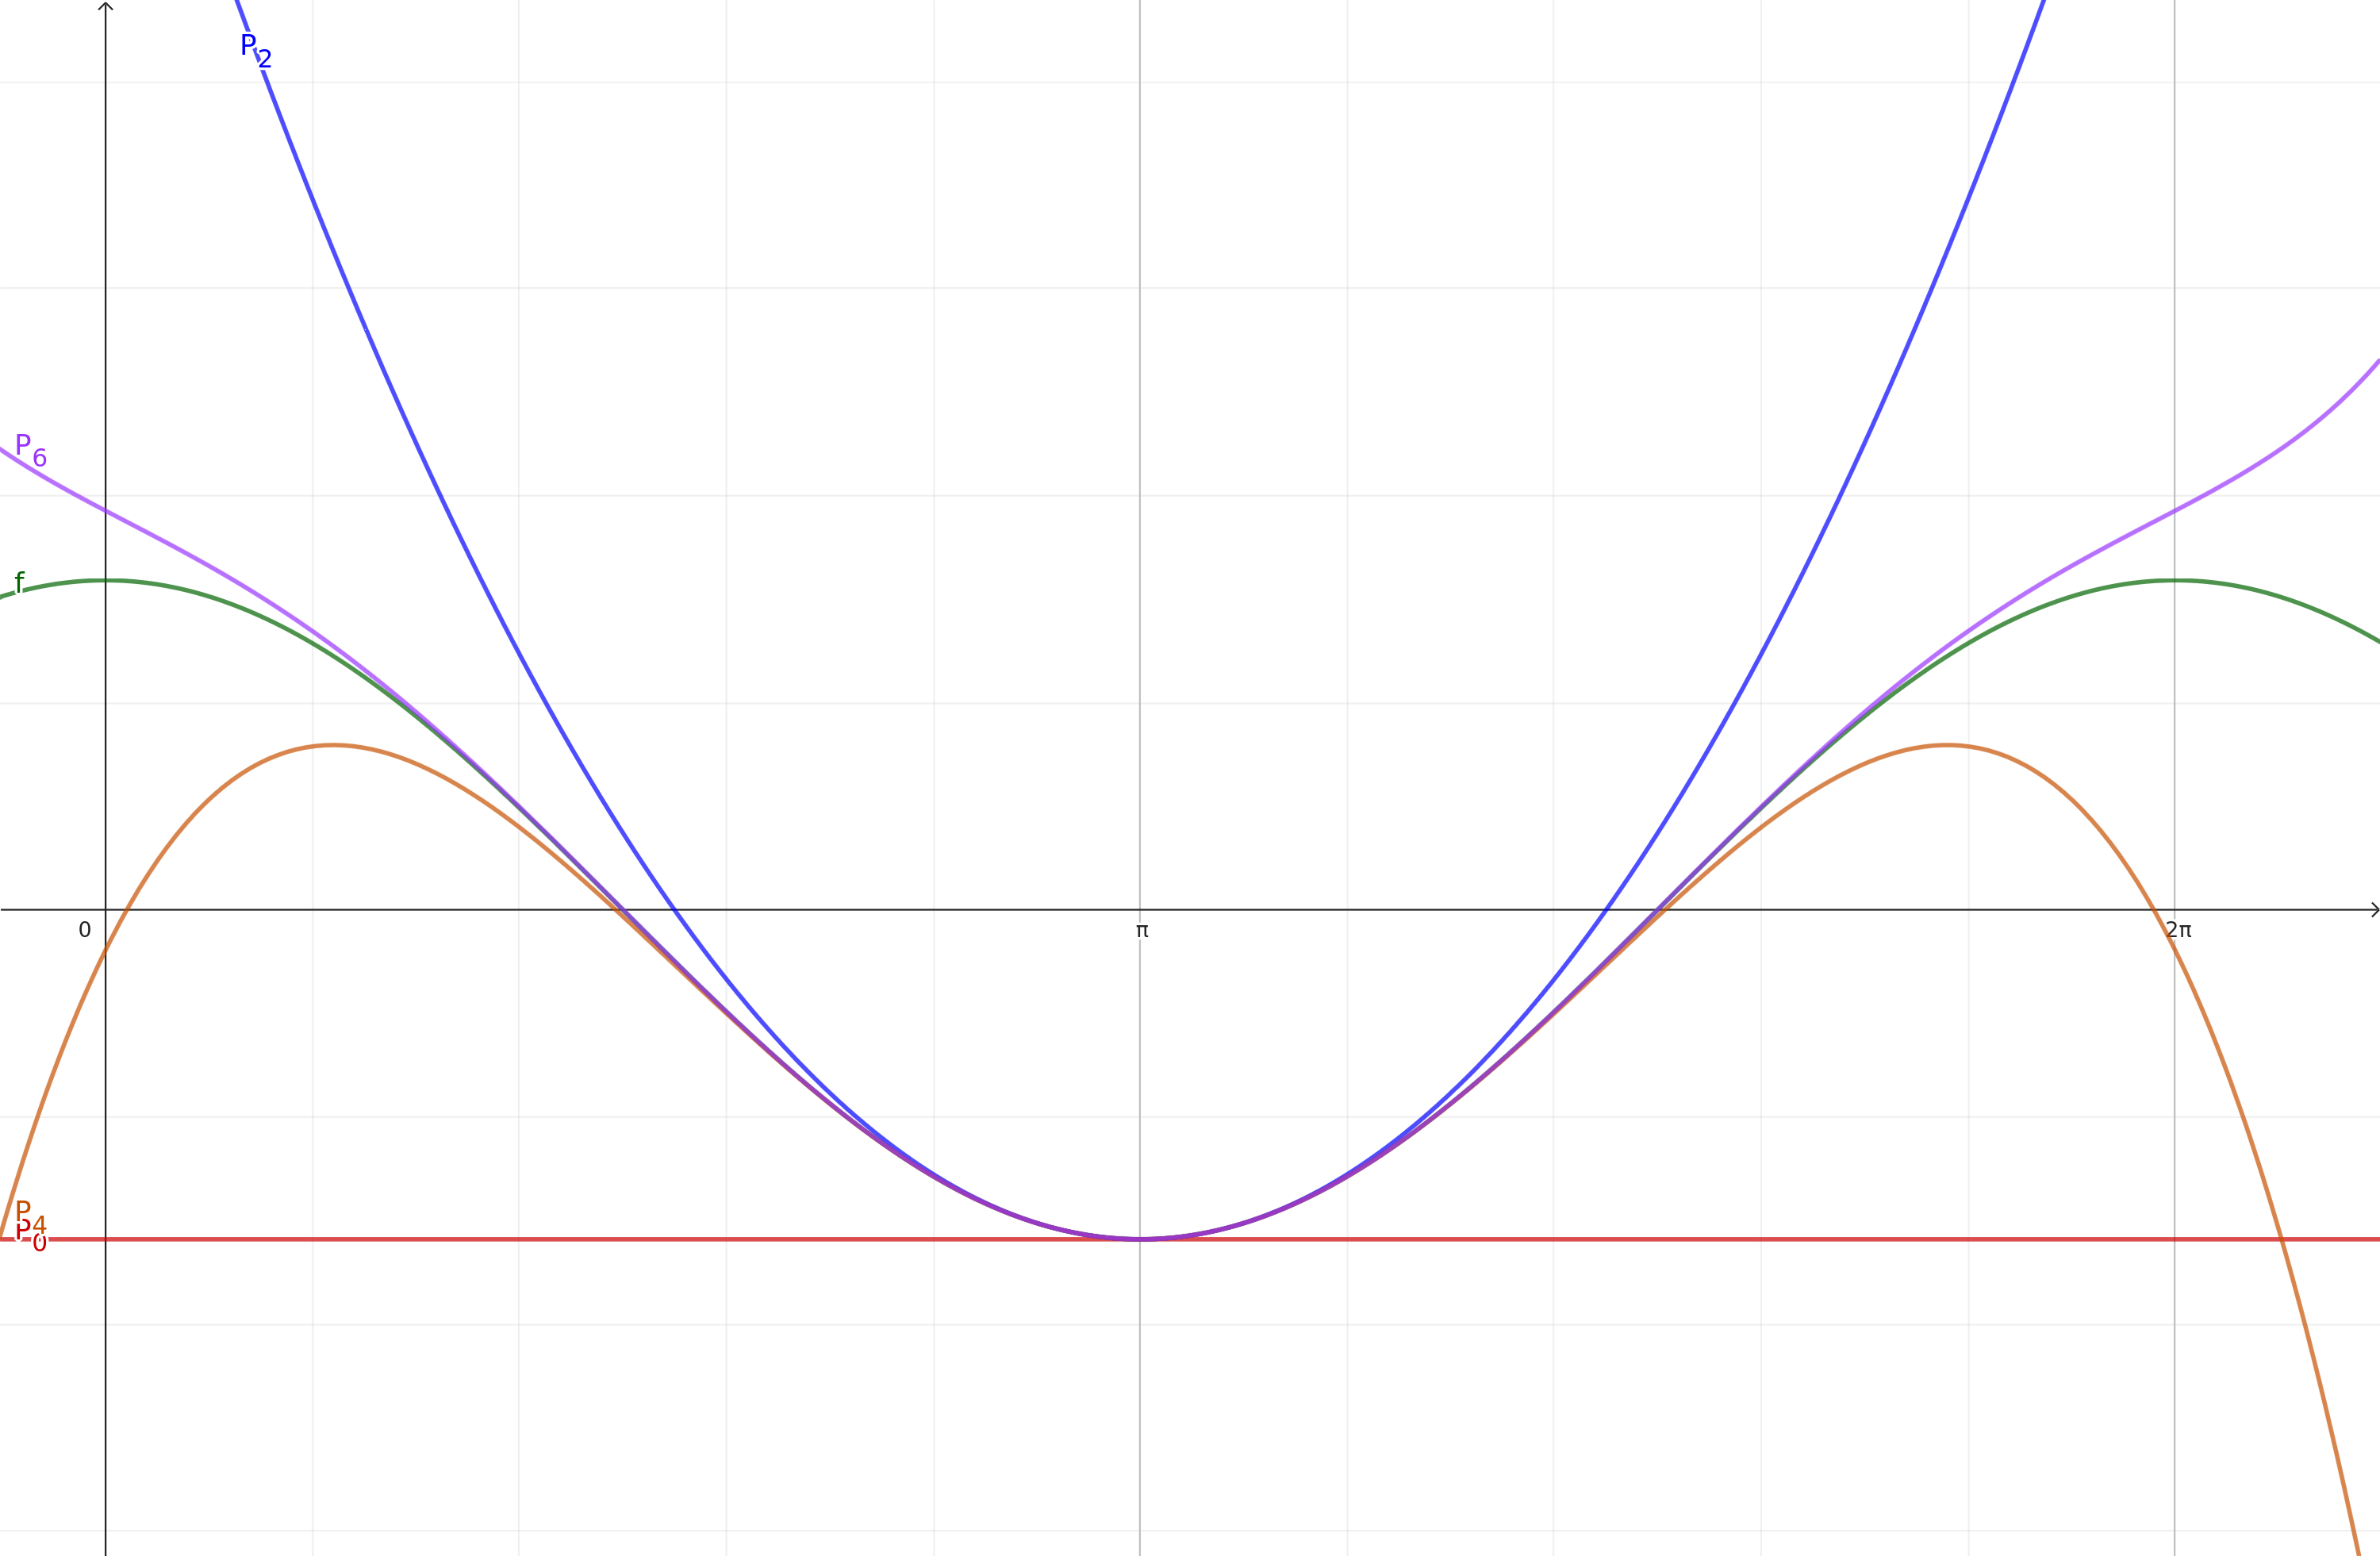
\includegraphics[height = 0.25\textheight]{recursos/polinomios/29zoom.png}\par
    \caption*{Ampliación de la Gráfica (Para notar mejor la aproximación realizada)}
    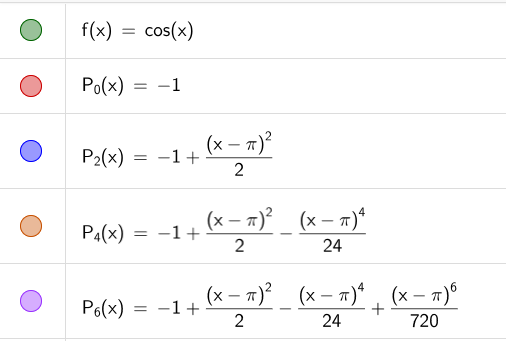
\includegraphics[height = 0.25\textheight]{recursos/polinomios/29Leyenda.png}\par
    \caption*{Simbología}
\end{figure*}